
\numberwithin{definition}{section}
\numberwithin{example}{section}
\numberwithin{equation}{section}
\numberwithin{figure}{section}

\addbibresource{../bib/taiga.bib}
\addbibresource{../bib/tex.bib}
%-----------------------------------------------------------------
\title{Regression costs for decision trees}
\author{\textsc{John Alan McDonald }}
\date{\today}
%-----------------------------------------------------------------
\begin{document}
\maketitle
%-----------------------------------------------------------------

The purpose of this document is work thru an alternative to $L_2$
cost that is a bit more efficient to compute, and gives the same
results when choosing split predicates in decision tree growing.

\section{\label{sub:Decision-trees}Greedy decision trees}

A general binary decision tree consists of
\begin{itemize}
\item internal \emph{split} nodes, each containing a predicate 
that determines
whether a record goes to the left or right child of that node.
\item terminal \emph{leaf} nodes, each containing a leaf model
 function whose value is the tree's prediction for any record 
 that ends up in that node. 
\end{itemize}

Greedy split optimization --- choose the best out of all
feasible splits, and repeat on the resulting child nodes until
there are no feasible splits --- is the most common way of
growing decision trees.
It depends on several things:
\begin{enumerate}
  \item A cost function $c$ used to define 'best'.  
  \item An enumeration of splits to consider. Pure greedy 
  splitting
  considers all 'feasible' splits on all attributes.
  \begin{enumerate} 
    \item For categorical attributes, that, in general, means 
    considering every partition of the categories into $2$ 
    subsets. However, for some important cost functions 
    (eg 2-class Gini, $L_2$), it can be shown that the optimal 
    split can be found by sorting the categories by the 
    corresponding score function (eg the response mean for $L_2$ 
    cost), and then considering only splits by score.
    \item For numerical attributes, the most general split would 
    come from treating the distinct values like the categories 
    of a categorical variable. However, no one does that, mostly 
    because there are usually too many distinct values. Instead, 
    only splits by
    $\leq$ vs $>$ one of the distinct values are considered.
\end{enumerate}
\item A feasibility test that determines whether a given split 
on a attribute is allowed. The most common case here is to 
require both children of the split contain some minimum number of 
training records.
\end{enumerate}

\section{\label{sec:numerical}Cost functions for $L_2$ numerical
regression}

Let $\mathcal{T} = \{ \left( y,\mathbf{x} \right) \}$ be the
training data in the node to be split.
It is a set of pairs of predictor record $\mathbf{x}$ and 
ground truth response $y$, where $y\in\mathbb{R}$ for numerical 
regression. We are considering splits on some particular 
predictor field $x_k$, which might be numerical or categorical.

The cost function for $L_2$ regression is the sum of squared 
deviations from the mean: 

$L_{2}\left(\mathcal{T}\right)
= \sum_{y\in\mathcal{T}}\,
\left(y-\bar{y}_{\mathcal{T}}\right)^{2}$,
where $\bar{y}_{\mathcal{T}}
= \frac{1}{\#\mathcal{T}}\sum_{y\in\mathcal{T}}\,y$.

Note that computing this \textit{accurately}, 
in an online fashion, for
moderate $\#\mathcal{T}$, the number of records in $\mathcal{T}$, 
allowing for
the updating/downdating needed for fast split optimization, 
requires some care. 

However, a little bit of algebra will let us use a simpler 
alternative to get the same splits. 


Any split partitions the training y-values
$\mathcal{T=}\left\{ y\right\} $ into left and right subsets: 
$\mathcal{T}=\mathcal{L}\uplus\mathcal{R}$.
The split cost is:

\begin{align*}
c\left(\mathcal{L},\mathcal{R}\right)= & 
L_{2}\left(\mathcal{L}\right)
+ L_{2}\left(\mathcal{R}\right)\\
= & \sum_{y\in\mathcal{L}}\,
\left(y-\bar{y}_{\mathcal{L}}\right)^{2}
+
\sum_{y\in\mathcal{R}}\,\left(y-\bar{y}_{\mathcal{R}}\right)^{2}\\
= & \sum_{y\in\mathcal{L}}\left[y^{2}-2\bar{y}_{\mathcal{L}}y
+
\bar{y}_{\mathcal{L}}^{2}\right]
+
\sum_{y\in\mathcal{R}}\left[y^{2}-2\bar{y}_{\mathcal{R}}y
+
\bar{y}_{\mathcal{R}}^{2}\right]\\
= & \sum_{\mathcal{L}\uplus\mathcal{R}}y^{2}
-
\frac{\left(\sum_{\mathcal{L}}y\right)^{2}}{\#\mathcal{L}}
-
\frac{\left(\sum_{\mathcal{R}}y\right)^{2}}{\#\mathcal{R}}
\end{align*}

Since $\sum_{\mathcal{L}\uplus\mathcal{R}}y^{2}$ doesn't 
depend on the split, minimizing 
$c\left(\mathcal{L},\mathcal{R}\right)$ is
equivalent to minimizing 
$-\left[\frac{\left(\sum_{\mathcal{L}}y\right)^{2}}{\#\mathcal{L}}
+
\frac{\left(\sum_{\mathcal{R}}y\right)^{2}}{\#\mathcal{R}}\right]$, 
so we can use 
$\frac{-\left(\sum_{\mathcal{T}}y\right)^{2}}{\#\mathcal{T}}$
as our cost function in split optimization.

\section{Cost functions for $L_2$ vector-valued regression}

Let $\mathcal{T} = \{ \left( \mathbf{y}, \mathbf{x} \right) \}$
be the training data in the node to be split.
Here the ground truth response $\mathbf{y}$ is a vector, 
$\mathbf{y}\in\mathbb{R}^m$, rather than a single number.

The cost function for $L_2$ vector-valued regression is the sum of
squared $L_2$ distances from the mean vector: 
\begin{align*}
L_{2}\left(\mathcal{T}\right) 
= &
\sum_{y\in\mathcal{T}}\,
\|\mathbf{y}-\bar{\mathbf{y}}_{\mathcal{T}}\|_{2}^{2}\\
= &
\sum_{y\in\mathcal{T}}\sum_{i=0}^{m-1}\,
\left(y_i-\bar{y_i}_{\mathcal{T}}\right)^{2}
\end{align*}

Following the same reasoning as in section~\ref{sec:numerical}, 
we get for a simpler cost:
$$
c\left(\mathcal{L},\mathcal{R}\right) = 
-\left[
\frac{
\sum_{i=0}^{m-1} \, \left(\sum_{\mathcal{L}}y_i\right)^{2}}
{\#\mathcal{L}}
\; + \;
\frac{\sum_{i=0}^{m-1} \,
\left(\sum_{\mathcal{R}}y_i\right)^{2}}{\#\mathcal{R}}\right] 
$$

\newpage{}
\section{Typesetting}

This document was typeset using Mik\TeX{} $2.9$ \cite{Miktex2017} 
and {\TeX}works $0.6.1$ \cite{Texworks2017} 
on \textsc{Windows} $10$. 
I used \texttt{arara} \cite{arara2017} 
to run \texttt{xelatex}, \texttt{biber}, \texttt{xelatex},  and
\texttt{xelatex}.
An alternative is to call these 4 commands by hand.

I believe only Mik\TeX\  and {\TeX}works are Windows specific; 
the actual typesetting tools should be usable on Linux and MacOS as well.

\begin{figure}[htbp]
\centering
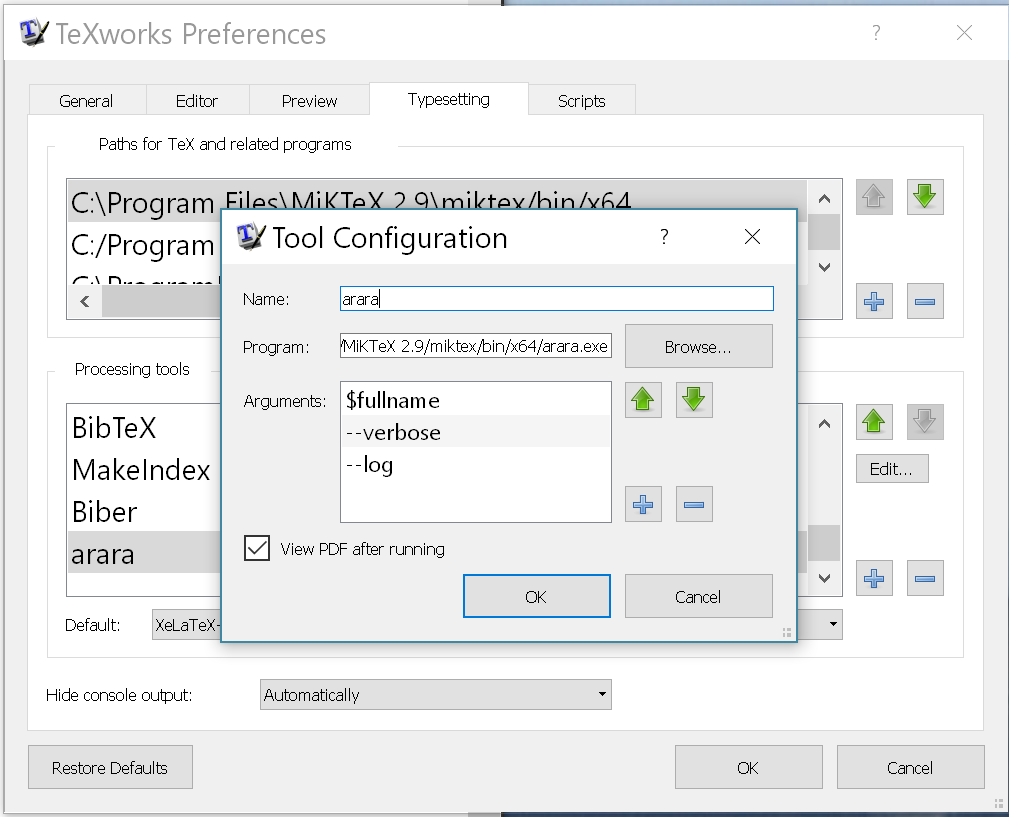
\includegraphics[scale=0.5]{../fig/arara.png}
\caption{Configuring {\TeX}works for \texttt{arara}.}
\label{fig:arara}
\end{figure}

%------------------------------------------------------------------------------
% \begingroup  % Temporarily disable \clearpage to show both lists on one page
%   %\let\clearpage\relax    % http://tex.stackexchange.com/a/14511/104449
%   \renewcommand{\listtheoremname}{List of definitions}
%   \textsf{\listoftheorems[ignoreall, show={definition}]}
% \endgroup
%-------------------------------------------------------------------------------
% \renewcommand{\listfigurename}{Figures}
% \addcontentsline{toc}{chapter}{\listfigurename}
% \begingroup
% \let\onecolumn\twocolumn
% \sffamily
% \listoffigures
% \rmfamily
% \endgroup
%-------------------------------------------------------------------------------
% \renewcommand{\lstlistlistingname}{Code samples}
% \addcontentsline{toc}{chapter}{\lstlistlistingname}
% \begingroup
% \let\onecolumn\twocolumn
% \sffamily
% \lstlistoflistings
% \rmfamily
% \endgroup
%-------------------------------------------------------------------------------
% \renewcommand{\listtheoremname}{Examples}
% \addcontentsline{toc}{chapter}{\lstlistlistingname}
% \begingroup
% \let\onecolumn\twocolumn
% \sffamily
% \listoftheorems
% \rmfamily
% \endgroup
%-------------------------------------------------------------------------------
% \newglossarystyle{mystyle}{%
%  \glossarystyle{altlist}%
%  \renewcommand*{\glossaryentryfield}[5]{%
%    \item[\glsentryitem{##1}\glstarget{##1}{##2}]%
%       :\hspace{1em}##3\glspostdescription\space ##5}%
% }
% \printglossary[title=Glossary,toctitle=Glossary]
%-------------------------------------------------------------------------------
\printbibliography[heading=bibintoc, title={References}]
%-------------------------------------------------------------------------------
% \printindex
%-------------------------------------------------------------------------------

\end{document}
